%%%%%%%% ICML 2026 EXAMPLE LATEX SUBMISSION FILE %%%%%%%%%%%%%%%%%

\documentclass{article}

% Recommended, but optional, packages for figures and better typesetting:
\usepackage{microtype}
\usepackage{graphicx}
\usepackage{subcaption}
\usepackage{booktabs} % for professional tables

% hyperref makes hyperlinks in the resulting PDF.
% If your build breaks (sometimes temporarily if a hyperlink spans a page)
% please comment out the following usepackage line and replace
% \usepackage{icml2026} with \usepackage[nohyperref]{icml2026} above.
\usepackage{hyperref}


% Attempt to make hyperref and algorithmic work together better:
\newcommand{\theHalgorithm}{\arabic{algorithm}}

% Use the following line for the initial blind version submitted for review:
\usepackage{icml2026}

% For preprint, use
% \usepackage[preprint]{icml2026}

% If accepted, instead use the following line for the camera-ready submission:
% \usepackage[accepted]{icml2026}

\usepackage{amsmath}
\usepackage{amssymb}
\usepackage{mathtools}
\usepackage{amsthm}


% if you use cleveref..
\usepackage[capitalize,noabbrev]{cleveref}

% ---- Packages ----
\usepackage{microtype}
\usepackage{graphicx}
\usepackage{subcaption}
\usepackage{booktabs}
\usepackage{multirow}
\usepackage{amsmath, amssymb, amsfonts}
\usepackage{mathtools}
\usepackage{bm}
\usepackage{algorithm}
\usepackage{algorithmic}
\usepackage{hyperref}
\usepackage{cleveref}
% \usepackage{enumitem}
\usepackage[inline, shortlabels]{enumitem}
\usepackage{xcolor}
\usepackage{amsthm}

% ---- Optional: TikZ for figures ----
\usepackage{tikz}
\usetikzlibrary{positioning, arrows.meta, calc}

% ---- Handy commands (edit later) ----
\newcommand{\wm}{\textsc{WM}}
\newcommand{\mawm}{\textsc{MAWM}}
\newcommand{\nsm}{\textsc{NS-MAWM}}
\newcommand{\DecPOMDP}{\textsc{Dec-POMDP}}
\newcommand{\RVR}{\textsc{RVR}}
\newcommand{\KL}{\mathrm{KL}}

\newcommand{\probP}{\text{I\kern-0.15em P}}

% Spell-checker exceptions for acronyms and domain-specific terms
% \usepackage{spellcheck}
% \spellcheck{MAWM,NS-MAWM,gridworld,SMAC,neuro-symbolic}

% --- Tickz
\usepackage{physics}
\usepackage{tikz}
\usetikzlibrary{arrows.meta,positioning,fit,calc}
\usepackage{amsmath}
\usepackage{mathdots}
% \usepackage{yhmath}
\usepackage{cancel}
\usepackage{color}
\usepackage{siunitx}
\usepackage{array}
\usepackage{stmaryrd}
\usepackage{multirow}
% \usepackage{amssymb}
\usepackage{gensymb}
\usepackage{tabularx}
\usepackage{extarrows}
\usepackage{booktabs}
\usetikzlibrary{fadings}
\usetikzlibrary{patterns}
\usetikzlibrary{shadows.blur}
\usetikzlibrary{shapes}

% ---- Math shortcuts ----
\newcommand{\E}{\mathbb{E}}
\newcommand{\R}{\mathbb{R}}
\newcommand{\I}{\mathbb{I}}

\usepackage{amssymb}
\usepackage{pifont}

\newcommand{\cmark}{\ding{51}}%
\newcommand{\xmark}{\ding{55}}%

\usepackage[english]{babel}
\addto\extrasenglish{  
    \def\figureautorefname{Figure}
    \def\tableautorefname{Table}
    \def\algorithmautorefname{Algorithm}
    \def\sectionautorefname{Section}
    \def\subsectionautorefname{Subsection}
    \def\proofoutlineautorefname{Proof Outline}
}

%%%%%%%%%%%%%%%%%%%%%%%%%%%%%%%%
% THEOREMS
%%%%%%%%%%%%%%%%%%%%%%%%%%%%%%%%
\theoremstyle{plain}
\newtheorem{theorem}{Theorem}[section]
\newtheorem{proposition}[theorem]{Proposition}
\newtheorem{lemma}[theorem]{Lemma}
\newtheorem{corollary}[theorem]{Corollary}
\theoremstyle{definition}
\newtheorem{definition}[theorem]{Definition}
\newtheorem{assumption}[theorem]{Assumption}
\theoremstyle{remark}
\newtheorem{remark}[theorem]{Remark}

% Todonotes is useful during development; simply uncomment the next line
%    and comment out the line below the next line to turn off comments
%\usepackage[disable,textsize=tiny]{todonotes}
\usepackage[textsize=tiny]{todonotes}

% The \icmltitle you define below is probably too long as a header.
% Therefore, a short form for the running title is supplied here:
\icmltitlerunning{Neuro-Symbolic Multi-Agent World Models}

\begin{document}

\twocolumn[
  \icmltitle{A Neuro-Symbolic Multi-Agent World Model Framework\\
    for Model-Based Multi-Agent Reinforcement Learning}

  % It is OKAY to include author information, even for blind submissions: the
  % style file will automatically remove it for you unless you've provided
  % the [accepted] option to the icml2026 package.

  % List of affiliations: The first argument should be a (short) identifier you
  % will use later to specify author affiliations Academic affiliations
  % should list Department, University, City, Region, Country Industry
  % affiliations should list Company, City, Region, Country

  % You can specify symbols, otherwise they are numbered in order. Ideally, you
  % should not use this facility. Affiliations will be numbered in order of
  % appearance and this is the preferred way.
  \icmlsetsymbol{equal}{*}

  \begin{icmlauthorlist}
    \icmlauthor{Julien Soulé}{equal,yyy}
    \icmlauthor{Georgios Bakirtzis}{equal,yyy,comp}
    \icmlauthor{Jean-Paul Jamont}{comp}
    \icmlauthor{Firstname4 Lastname4}{sch}
    \icmlauthor{Firstname5 Lastname5}{yyy}
    \icmlauthor{Firstname6 Lastname6}{sch,yyy,comp}
    \icmlauthor{Firstname7 Lastname7}{comp}
    %\icmlauthor{}{sch}
    \icmlauthor{Firstname8 Lastname8}{sch}
    \icmlauthor{Firstname8 Lastname8}{yyy,comp}
    %\icmlauthor{}{sch}
    %\icmlauthor{}{sch}
  \end{icmlauthorlist}

  \icmlaffiliation{yyy}{Department of XXX, University of YYY, Location, Country}
  \icmlaffiliation{comp}{Company Name, Location, Country}
  \icmlaffiliation{sch}{School of ZZZ, Institute of WWW, Location, Country}

  \icmlcorrespondingauthor{Julien Soulé}{julien.soule@hotmail.fr}
  \icmlcorrespondingauthor{Firstname2 Lastname2}{first2.last2@www.uk}

  % You may provide any keywords that you find helpful for describing your
  % paper; these are used to populate the "keywords" metadata in the PDF but
  % will not be shown in the document
  \icmlkeywords{Machine Learning, ICML}

  \vskip 0.3in
]

% this must go after the closing bracket ] following \twocolumn[ ...

% This command actually creates the footnote in the first column listing the
% affiliations and the copyright notice. The command takes one argument, which
% is text to display at the start of the footnote. The \icmlEqualContribution
% command is standard text for equal contribution. Remove it (just {}) if you
% do not need this facility.

% Use ONE of the following lines. DO NOT remove the command.
% If you have no special notice, KEEP empty braces:
\printAffiliationsAndNotice{}  % no special notice (required even if empty)
% Or, if applicable, use the standard equal contribution text:
% \printAffiliationsAndNotice{\icmlEqualContribution}

% ============================
% Abstract
% ============================
\begin{abstract}
  Model-based reinforcement learning enables planning through learned WMs, but extending these approaches to multi-agent settings is challenging due to partial observability and error accumulation in joint observation dynamics. Purely neural multi-agent WMs often produce semantically inconsistent predictions, violating spatial coherence, object persistence, and interaction constraints.
  We introduce \textbf{Neuro-Symbolic Multi-Agent WMs (NS-MAWM)}, which incorporate symbolic invariants and action-conditioned equivariances as differentiable consistency constraints during WM training. These constraints act as structured inductive biases that reduce long-horizon semantic drift.
  We evaluate NS-MAWM on four representative multi-agent environments with three proposed neuro-symbolic integration strategies. Experimental results show that NS-MAWM improves long-horizon prediction consistency, planning performance, and generalization compared to a purely neural baseline.
\end{abstract}

% ============================
% 1. Introduction
% ============================
\section{Introduction}
\label{sec:intro}

Learning predictive models of environment dynamics, known as \emph{WMs} (WMs)~\cite{ha2018worldmodels}, is a central paradigm in model-based reinforcement learning (MBRL)~\cite{hafner2019learning,hafner2020dreamer,hafner2021dreamerv2}. By encoding the agent's interaction history into a latent space, these models enable imagination-based planning, policy learning, and long-horizon credit assignment~\cite{schrittwieser2020}. Recent progress in this area has shown strong results in single-agent and fully observable environments; however, their extension to multi-agent settings with partial observability remains an open frontier~\cite{Wong2023,Venugopal2024MABL,agravante-etal-2023-learning}.

In such environments, observations typically consist of multiple interacting entities governed by spatial, logical, or physical rules (for instance two agents cannot occupy the same location, objects follow deterministic transitions, etc.). Yet, most WMs treat observations as flat, unstructured vectors~\cite{ha2018worldmodels,hafner2019learning}, and learn monolithic latent dynamics end-to-end from raw pixels. This often leads to latent representations that fail to disentangle semantics (such as agent identity, object types) or to reflect the compositional structure of the environment~\cite{kipf2020contrastivelearningstructuredworld,bronstein2021geometric}. As a result, models may produce high-likelihood predictions that are logically inconsistent or physically implausible.

For instance, a trained WM might predict that two agents occupy the same grid cell, violating collision rules. Such symbolic inconsistencies are not penalized by standard likelihood or reconstruction losses, often going unnoticed during evaluation. Worse, these errors compound during long rollouts, degrading planning performance and breaking environment logic~\cite{talvitie2014modelbias,venkatraman2015improving}.

Several works have pioneered the incorporation of prior knowledge as inductive biases into WMs~\cite{kipf2020contrastivelearningstructuredworld,mondal2022eqr}. However, a general framework for integrating symbolic reasoning into WMs learning has yet to be established, especially regarding three general gaps:
%
\begin{itemize}
  \item[\textbf{G1}] \textbf{Lack of Multi-Agent-Oriented WM Structures.}
    Existing WMs neglect structural priors for multi-agent environments: explicit representation of partial observability, interaction-induced non-stationarity, and entity modularity~\cite{zhang2021worldmodelgraph, Willemsen2021MAMBPO, Venugopal2024MABL}. They assume stationary dynamics and treat agents uniformly, failing to generalize across varied configurations.

  \item[\textbf{G2}] \textbf{Lack of Neuro-Symbolic Integration in WMs.}
    While symbolic priors (action constraints, physical laws, interaction rules) enhance sample efficiency and robustness, few models incorporate them into WM learning or architecture~\cite{Xu2018semanticloss, Fan2017differentiablelearninglogicalrules, balloch2023neurosymbolicworldmodelsadapting, garcez2023neurosymbolic}. Most rely solely on black-box latent dynamics, missing opportunities to leverage symbolic knowledge as inductive bias.

  \item[\textbf{G3}] \textbf{Lack of Symbolic Coherence as an Optimization Principle.}
    Standard WM metrics focus on predictive accuracy or downstream reward, overlooking symbolic consistency. Yet reasoning in dynamic environments benefits from verifying whether predictions respect constraints~\cite{talvitie2014modelbias, balloch2023neurosymbolicworldmodelsadapting}.
\end{itemize}

Building on neuro-symbolic integration frameworks~\cite{manhaeve2018deepproblog,garcez2023neurosymbolic,Xu2018semanticloss,Fan2017differentiablelearninglogicalrules}, we propose \textbf{NS-MAWM} to augment WMs with symbolic reasoning through:
%
\begin{itemize}
  \item A \emph{structured latent space} that decomposes observations into typed entities (agents, objects) with interpretable attributes (such as position or type), enabling effective symbolic rule application.

  \item A \emph{symbolic rule formalism} that expresses environment dynamics as differentiable constraints over observations and actions, clearly specifying invariants and action-conditioned equivariances.

  \item Three neuro-symbolic integration strategies:
        \begin{enumerate*}[label={\roman*) },itemjoin={; \quad}]
          \item \textbf{Symbolic Loss Regularization}: rules are encoded as differentiable soft constraints, similarly to semantic loss or logic regularization frameworks
          \item \textbf{Symbolic Projection}: violations are corrected by projecting predictions to valid configurations, ensuring adherence to the defined rules.
          \item \textbf{Residual Symbolic Dynamics}: transitions are factorized into a symbolic process and learned residuals, allowing for a more accurate approach to learning.
        \end{enumerate*}

  \item A \emph{Rule Violation Rate (RVR)} metric that quantifies constraint violations for logical consistency evaluation.
\end{itemize}

We evaluate NS-MAWM across four discrete and continuous environments: a proposed Minecraft-like gridworld, Overcooked~\cite{Micah2020overcooked}, a Predator-Prey environment~\cite{lowe2017multi} and the SMAC environment~\cite{Ellis2023smacv2}. Our comparison includes various integration strategies alongside a vanilla WM baseline, utilizing both standard and symbolic metrics for assessment. The results demonstrate that NS-MAWM not only improves prediction accuracy but also enhances generalization to new configurations, significantly reducing symbolic violations. Among the integration strategies, for similar performance, the residual symbolic dynamics strategy shows the fastest convergence, while the combination of the symbolic loss regularization strategy and the symbolic projection one provide stronger coherence over longer time horizons.

The remainder of the paper is organized as follows: \autoref{sec:related_work} surveys related work, \autoref{sec:background} briefly reviews background concepts, \autoref{sec:method} details NS-MAWM, \autoref{sec:eval} presents experiments, and \autoref{sec:conclusion} concludes.



% ============================
% 3. Related Work
% ============================

\section{Related Work}
\label{sec:related_work}
% TODO: On cherche les travaux qui permettent d'avoir un WM qui permette une meilleure prise en compte de :
%  - l'observabilité partielle,
%  - de la non-stationnarité (autres agents qui interagissent en même temps),
%  - l'aspect multi-agent dans l'architecture du modèle,
%  - l'interpretation des observations en particulier au regard d'un environnement multi-agent complexe
%  - la possibilité d'injecter des règles symboliques
%  - la possibilité d'évaluer la cohérence au regard des règles symboliques
%  - la robustesse à des variations de l'environnement
%  - la généralisation à de nouvelles configurations d'agents/objets
%  - l'efficacité en termes de temps de calcul et de données pour converger vers une performance comparable par rapport à un WM classique (la frugalité du temps de calcul)
%  - la frugalité en termes de données (moins de données nécessaires pour atteindre une certaine performance)
%  - la scalabilité avec le nombre d'agents/objets/règles
%  - le drift sémantique sur le long terme (est-ce que le modèle reste cohérent sur le long terme ?)

We review the landscape of related works across four major axes of relevance to NS-MAWM:

\paragraph{Architectures of World Models.} Early approaches such as Dreamer~\cite{hafner2020dreamer, hafner2021dreamerv2} and PlaNet~\cite{hafner2019learning} proposed powerful black-box latent dynamics models, often using a monolithic latent space without architectural bias toward entities or agents. More recent efforts adopt a structured representation. For instance, World Model as Graph~\cite{zhang2021worldmodelgraph} and MABL~\cite{Venugopal2024MABL} propose latent modularity aligned with environment entities and topology. MAMBPO~\cite{Willemsen2021MAMBPO} incorporates explicit multi-agent structure, allowing rollouts conditioned on individual agent views.

\paragraph{Learning in Multi-Agent Environments.} Some models simply treat other agents as part of the environment, hence implicitly stationary. Mingling Foresight~\cite{Xu2022mingling} and Multi-Timescale MARL~\cite{nekoei2023dealing} improve handling of concurrent interactions via hierarchical reasoning or timescale adaptation. Opponent modeling is tackled explicitly in~\cite{Yuxiaopeng2022modelbased}, which proposes world models conditioned on latent opponent policies.

\paragraph{Symbolic Knowledge in World Models.} Symbolic priors are sparsely represented in world model literature. Several efforts inject domain knowledge as constraints, such as Semantic Loss~\cite{Xu2018semanticloss} and differentiable logic rules~\cite{Fan2017differentiablelearninglogicalrules}. DeepProbLog~\cite{manhaeve2018deepproblog} merges probabilistic logic with deep models. Recent neuro-symbolic world models~\cite{balloch2023neurosymbolicworldmodelsadapting, agravante-etal-2023-learning} propose explicit symbolic structure over latent dynamics to support adaptation and interpretability.

\paragraph{Evaluation Dimensions.} Most WMs are evaluated using reconstruction loss or control performance, but few assess coherence with symbolic rules or generalization under structural shifts. Some recent benchmarks~\cite{Duan_2025_ICCV} and surveys~\cite{Wong2023, Delvecchio2025p1157} advocate for broader evaluation metrics, including semantic consistency, rule violation rates, and frugality in data/time.

\begin{table*}[t]
  \centering
  \resizebox{\textwidth}{!}{%
    \footnotesize
    \begin{tabular}{p{4.69cm}cccccccc}
      \toprule
      \textbf{Work}                                                  & Struct. WM & MA-aware & NS-aware & Symb. Priors & Symb. Coher. & Robust & Gen.   & Frugal \\
      \midrule
      Dreamer~\cite{hafner2020dreamer}                               & \xmark     & \xmark   & \xmark   & \xmark       & \xmark       & \xmark & $\sim$ & $\sim$ \\
      WM as Graph~\cite{zhang2021worldmodelgraph}                    & \cmark     & $\sim$   & \xmark   & \xmark       & \xmark       & \xmark & $\sim$ & \xmark \\
      MABL~\cite{Venugopal2024MABL}                                  & \cmark     & \cmark   & $\sim$   & \xmark       & \xmark       & $\sim$ & \cmark & $\sim$ \\
      MAMBPO~\cite{Willemsen2021MAMBPO}                              & \cmark     & \cmark   & \xmark   & \xmark       & \xmark       & \xmark & $\sim$ & \cmark \\
      WorldCloner~\cite{balloch2023neurosymbolicworldmodelsadapting} & \cmark     & \cmark   & \cmark   & \cmark       & \cmark       & $\sim$ & \cmark & \xmark \\
      Mingling~\cite{Xu2022mingling}                                 & $\sim$     & \cmark   & \cmark   & \xmark       & \xmark       & \cmark & \cmark & \cmark \\
      OppMod~\cite{Yuxiaopeng2022modelbased}                         & \xmark     & \cmark   & \cmark   & \xmark       & \xmark       & $\sim$ & $\sim$ & \xmark \\
      DeepProbLog~\cite{manhaeve2018deepproblog}                     & \xmark     & \xmark   & \xmark   & \cmark       & \xmark       & \xmark & \xmark & \xmark \\
      NS-WM~\cite{agravante-etal-2023-learning}                      & \cmark     & \cmark   & $\sim$   & \cmark       & \cmark       & $\sim$ & $\sim$ & \xmark \\
      \bottomrule
    \end{tabular}
  }
  \caption{Comparison of representative works. Struct. WM: structured world model; MA-aware: multi-agent awareness; NS-aware: non-stationarity; Symb. Priors: symbolic priors; Symb. Coher.: symbolic coherence evaluation; Robust: robustness; Gen.: generalization; Frugal: data/time efficiency.}
  \label{tab:related_work}
\end{table*}

\autoref{tab:related_work} summarizes this landscape, highlighting how existing works address (or neglect) the critical dimensions we target. Despite significant progress, most existing world models fail to simultaneously address the three critical dimensions we target. Specifically, they often lack : (\textbf{G1}) multi-agent specific architectural bias, (\textbf{G2}) integration of symbolic priors or reasoning mechanisms, and (\textbf{G3}) coherence verification against symbolic knowledge. These gaps motivate our proposed framework to support structured, interpretable, and efficient learning in multi-agent partially observable environments with evolving dynamics.


\section{Background and basics}
\label{sec:background}

\subsection{MARL framework}
\label{sec:decpomdp}

To apply MARL techniques, we rely on the \textit{Decentralized Partially Observable Markov Decision Process} (Dec-POMDP) \cite{Oliehoek2016}. Dec-POMDPs naturally model decentralized multi-agent coordination under partial observability, making them well suited for integrating organizational constraints. Unlike \textit{Partially Observable Stochastic Games} (POSG), the Dec-POMDP allows for a common reward function for agents, which promotes collaboration~\cite{Beynier2013}.

A Dec-POMDP $d \in D$ (where $D$ is the set of Dec-POMDPs) is defined as a 7-tuple $d = \langle S, \{A_i\}, T, R, \{\Omega_i\}, O, \gamma \rangle$, where $S = \{s_1,\dots,s_{|S|}\}$ is the set of possible states; $A_{i} = \{a_{1}^{i},\dots,a_{|A_{i}|}^{i}\}$ is the set of possible actions for agent $i$; $T$ represents the set of transition probabilities, with $T(s,a,s') = \probP(s'|s,a)$ as the probability of transitioning from state $s$ to state $s'$ following action $a$; $R: S \times A \times S \rightarrow \mathbb{R}$ is the reward function, assigning a reward based on the initial state, the action taken, and the resulting state; $\Omega_{i} = \{o_{1}^{i},\dots,o_{|\Omega_{i}|}^{i}\}$ is the set of possible observations for agent $i$; $O$ represents the set of observation probabilities, where $O(s',a,o) = \probP(o|s',a)$ is the probability of obtaining observation $o$ after performing action $a$ and reaching state $s'$; and $\gamma \in [0,1]$ is the discount factor
%, used to weight future rewards.

The following formalism is used to solve the Dec-POMDP~\cite{Beynier2013,Albrecht2024}: $\mathcal{A}$ represents the set of $n$ \textbf{agents}; $\Pi$ denotes the set of \textbf{policies}, where a policy $\pi \in \Pi, \pi: \Omega \rightarrow A$ deterministically maps an observation to an action, representing the agent's internal strategy; $\Pi_{joint}$ represents the set of \textbf{joint policies}, with a joint policy $\pi_{joint} \in \Pi_{joint}, \pi_{joint}: \Omega^n \rightarrow A^n = \Pi^n$, which selects an action for each agent based on their respective observations, acting as a collection of policies used by agents within a team; $H$ is the set of \textbf{histories}, where a history (or trajectory) over $z \in \mathbb{N}$ steps (typically the maximum number of steps in an episode) is represented as the $z$-tuple $h = \langle \langle \omega_{k}, a_{k}\rangle | k \leq z, \omega \in \Omega, a \in A\rangle$, capturing successive observations and actions; $H_{joint}$ stands for the set of \textbf{joint histories}, with a joint history $h_{joint} \in H_{joint}$ over $z$ steps defined as the set of agent histories: $h_{joint} = \{h_1, h_2, \dots, h_n\}$; and finally, $V_{joint}(\pi_{joint}): \Pi_{joint} \rightarrow \mathbb{R}$ denotes the \textbf{expected cumulative reward} over a finite horizon (assuming $\gamma < 1$ or if the number of steps in an episode is finite), where $\pi_{joint}$ represents the joint policy for team $i$, with $\pi_{joint,-i}$ being the joint policies of other teams, considered as fixed.

\subsection{Model-Based MARL}
\label{sec:mb-marl}

TODO

\subsection{The WM basics}
\label{sec:wm_basics}

In \textbf{RL}, and particularly under partial observability, \textbf{WMs}~\cite{ha2018worldmodels, hafner2020dreamer} aim to learn internal models that jointly approximate both transition and observation dynamics. \textit{WMs} enable agents to perform planning, improve sample efficiency, and facilitate safe exploration by allowing the agent to simulate future scenarios. This approach belongs to the \textbf{MBRL} paradigm~\cite{moerland2020model}, and proves particularly useful for automatically constructing high-fidelity simulation models even in the absence of an explicit environment representation.

Formally, at each time step $t$, let $\omega_t \in \Omega$ denote the current observation, $a_t \in A$ the executed action, and $\tilde{h}_{t-1} \in \mathcal{H}$ the recurrent hidden state summarizing the interaction history up to $t-1$. Since observations are generally high-dimensional (e.g., images or complex state vectors), an encoder $Enc: \Omega \rightarrow Z$ is applied to project observations into a compact latent space $Z$, with $z_t = Enc(\omega_t)$, where $\dim(Z) \ll \dim(\Omega)$.

The main temporal structure is modeled using a \textbf{Recurrent Latent Dynamics Model (\textbf{RLDM})}~\cite{hafner2020dreamer} $\mathcal{T}^{z} = f(g(h_{t-1}, z_t, a_t))$, which predicts the next latent state $\hat{z}_{t+1}$ by updating the recurrent state via $f$ and applying latent dynamics via $g$:
\[
  h_t = f(h_{t-1}, z_t, a_t), \quad \hat{z}_{t+1} = g(h_t)
\]
where $f(\cdot)$ typically corresponds to a recurrent neural network \textbf{Recurrent Neural Network} (RNN) such as a \textbf{Long Short-Term Memory}~\cite{hochreiter1997long} (LSTM), applied to the concatenation of $h_{t-1}$, $z_t$, and $a_t$, and $g(\cdot)$ is a function (often implemented as an \textbf{MLP}) mapping the recurrent state to the latent representation of the next observation.

The predicted latent state is then decoded by $Dec: Z \rightarrow \Omega$ to produce the predicted observation $\hat{\omega}_{t+1} = Dec(\hat{z}_{t+1})$. The entire model is trained jointly to minimize both the \emph{reconstruction loss} $\|\omega_{t+1} - \hat{\omega}_{t+1}\|$ in observation space, and optionally a \emph{latent prediction loss} to stabilize learning of the latent dynamics.

The recurrent hidden state $\tilde{h}_t$ serves as a compact summary of the complete interaction history up to time $t$, thus avoiding the need to explicitly store long observation-action sequences.

For conciseness, we define the full composition that directly maps the current observation, action, and recurrent state to the next predicted observation as the \textbf{Observation Prediction Model} (\textbf{OPM}):
\begin{align*}
  \mathcal{T}(h_{t-1}, \omega_t, a_t) := Dec(g(f(h_{t-1}, Enc(\omega_t), a_t))) = \hat{\omega}_{t+1}
\end{align*}

\begin{figure}[h!]
  \centering
  \resizebox{\columnwidth}{!}{%
    


\tikzset{every picture/.style={line width=0.75pt}} %set default line width to 0.75pt        

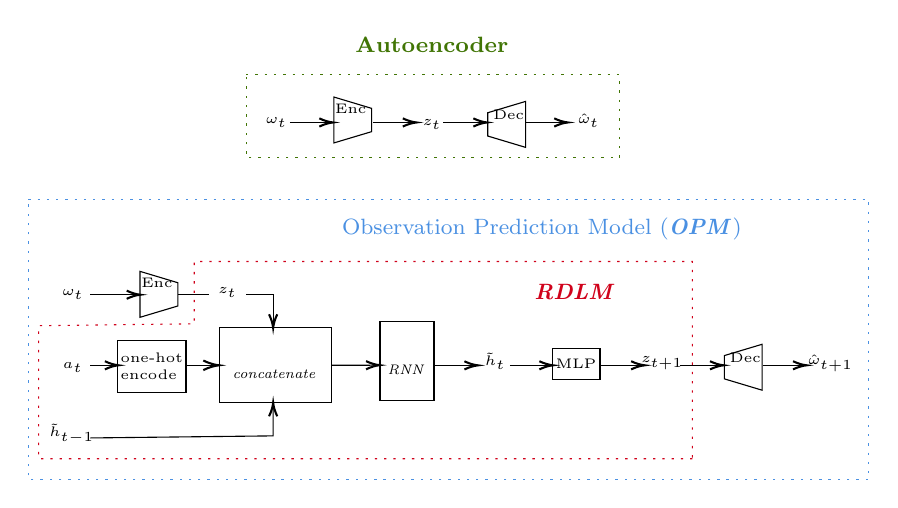
\begin{tikzpicture}[x=0.75pt,y=0.75pt,yscale=-1,xscale=1]
    %uncomment if require: \path (0,2102); %set diagram left start at 0, and has height of 2102

    %Straight Lines [id:da7945271061326031] 
    \draw    (100,1800) -- (111.5,1800) ;
    \draw [shift={(113.5,1800)}, rotate = 180] [color={rgb, 255:red, 0; green, 0; blue, 0 }  ][line width=0.75]    (6.56,-1.97) .. controls (4.17,-0.84) and (1.99,-0.18) .. (0,0) .. controls (1.99,0.18) and (4.17,0.84) .. (6.56,1.97)   ;
    %Straight Lines [id:da710289636295716] 
    \draw    (100,1835) -- (188,1834) -- (188,1820) ;
    \draw [shift={(188,1818)}, rotate = 90] [color={rgb, 255:red, 0; green, 0; blue, 0 }  ][line width=0.75]    (6.56,-1.97) .. controls (4.17,-0.84) and (1.99,-0.18) .. (0,0) .. controls (1.99,0.18) and (4.17,0.84) .. (6.56,1.97)   ;
    %Straight Lines [id:da9775676154282154] 
    \draw    (146.38,1800) -- (160,1800) ;
    \draw [shift={(162,1800)}, rotate = 180] [color={rgb, 255:red, 0; green, 0; blue, 0 }  ][line width=0.75]    (7.65,-2.3) .. controls (4.86,-0.97) and (2.31,-0.21) .. (0,0) .. controls (2.31,0.21) and (4.86,0.98) .. (7.65,2.3)   ;
    %Straight Lines [id:da789934339782699] 
    \draw    (100,1766) -- (122,1766) ;
    \draw [shift={(124,1766)}, rotate = 180] [color={rgb, 255:red, 0; green, 0; blue, 0 }  ][line width=0.75]    (6.56,-1.97) .. controls (4.17,-0.84) and (1.99,-0.18) .. (0,0) .. controls (1.99,0.18) and (4.17,0.84) .. (6.56,1.97)   ;
    %Shape: Trapezoid [id:dp2317709974845179] 
    \draw   (123.84,1754.74) -- (142.07,1760.21) -- (142.07,1771.42) -- (123.84,1776.88) -- cycle ;
    %Straight Lines [id:da7383754609221514] 
    \draw    (142,1766) -- (188,1766) -- (188,1780) ;
    \draw [shift={(188,1782)}, rotate = 270] [color={rgb, 255:red, 0; green, 0; blue, 0 }  ][line width=0.75]    (6.56,-1.97) .. controls (4.17,-0.84) and (1.99,-0.18) .. (0,0) .. controls (1.99,0.18) and (4.17,0.84) .. (6.56,1.97)   ;
    %Straight Lines [id:da49394763541143527] 
    \draw    (216,1800) -- (237.33,1799.94) ;
    \draw [shift={(239.33,1799.94)}, rotate = 179.85] [color={rgb, 255:red, 0; green, 0; blue, 0 }  ][line width=0.75]    (6.56,-1.97) .. controls (4.17,-0.84) and (1.99,-0.18) .. (0,0) .. controls (1.99,0.18) and (4.17,0.84) .. (6.56,1.97)   ;
    %Straight Lines [id:da8738633046359771] 
    \draw    (265.89,1800.03) -- (284.72,1800.03) ;
    \draw [shift={(286.72,1800.03)}, rotate = 180] [color={rgb, 255:red, 0; green, 0; blue, 0 }  ][line width=0.75]    (6.56,-1.97) .. controls (4.17,-0.84) and (1.99,-0.18) .. (0,0) .. controls (1.99,0.18) and (4.17,0.84) .. (6.56,1.97)   ;
    %Straight Lines [id:da3021616845453272] 
    \draw    (302,1800) -- (320.83,1800) ;
    \draw [shift={(322.83,1800)}, rotate = 180] [color={rgb, 255:red, 0; green, 0; blue, 0 }  ][line width=0.75]    (6.56,-1.97) .. controls (4.17,-0.84) and (1.99,-0.18) .. (0,0) .. controls (1.99,0.18) and (4.17,0.84) .. (6.56,1.97)   ;
    %Straight Lines [id:da8984410115217915] 
    \draw    (346,1800) -- (353.4,1800) -- (365.04,1800) ;
    \draw [shift={(367.04,1800)}, rotate = 180] [color={rgb, 255:red, 0; green, 0; blue, 0 }  ][line width=0.75]    (6.56,-1.97) .. controls (4.17,-0.84) and (1.99,-0.18) .. (0,0) .. controls (1.99,0.18) and (4.17,0.84) .. (6.56,1.97)   ;
    %Shape: Trapezoid [id:dp37639710819638017] 
    \draw   (423.61,1812) -- (405.38,1806.53) -- (405.38,1795.32) -- (423.61,1789.86) -- cycle ;
    %Straight Lines [id:da10289425963982124] 
    \draw    (384,1800) -- (403.04,1800) ;
    \draw [shift={(405.04,1800)}, rotate = 180] [color={rgb, 255:red, 0; green, 0; blue, 0 }  ][line width=0.75]    (6.56,-1.97) .. controls (4.17,-0.84) and (1.99,-0.18) .. (0,0) .. controls (1.99,0.18) and (4.17,0.84) .. (6.56,1.97)   ;
    %Straight Lines [id:da12692360321469986] 
    \draw    (424,1800) -- (443.04,1800) ;
    \draw [shift={(445.04,1800)}, rotate = 180] [color={rgb, 255:red, 0; green, 0; blue, 0 }  ][line width=0.75]    (6.56,-1.97) .. controls (4.17,-0.84) and (1.99,-0.18) .. (0,0) .. controls (1.99,0.18) and (4.17,0.84) .. (6.56,1.97)   ;
    %Shape: Trapezoid [id:dp27180057752038367] 
    \draw   (217.23,1670.74) -- (235.46,1676.21) -- (235.46,1687.42) -- (217.23,1692.88) -- cycle ;
    %Shape: Trapezoid [id:dp9437628483591106] 
    \draw   (309.61,1695) -- (291.38,1689.53) -- (291.38,1678.32) -- (309.61,1672.86) -- cycle ;
    %Straight Lines [id:da19635385567867214] 
    \draw    (310,1683) -- (328,1683) ;
    \draw [shift={(330,1683)}, rotate = 180] [color={rgb, 255:red, 0; green, 0; blue, 0 }  ][line width=0.75]    (6.56,-1.97) .. controls (4.17,-0.84) and (1.99,-0.18) .. (0,0) .. controls (1.99,0.18) and (4.17,0.84) .. (6.56,1.97)   ;
    %Straight Lines [id:da6136759960935583] 
    \draw    (196,1683) -- (214.83,1683) ;
    \draw [shift={(216.83,1683)}, rotate = 180] [color={rgb, 255:red, 0; green, 0; blue, 0 }  ][line width=0.75]    (6.56,-1.97) .. controls (4.17,-0.84) and (1.99,-0.18) .. (0,0) .. controls (1.99,0.18) and (4.17,0.84) .. (6.56,1.97)   ;
    %Straight Lines [id:da5198115307428596] 
    \draw    (236,1683) -- (255.04,1683) ;
    \draw [shift={(257.04,1683)}, rotate = 180] [color={rgb, 255:red, 0; green, 0; blue, 0 }  ][line width=0.75]    (6.56,-1.97) .. controls (4.17,-0.84) and (1.99,-0.18) .. (0,0) .. controls (1.99,0.18) and (4.17,0.84) .. (6.56,1.97)   ;
    %Straight Lines [id:da6362560665768464] 
    \draw    (270,1683) -- (289.04,1683) ;
    \draw [shift={(291.04,1683)}, rotate = 180] [color={rgb, 255:red, 0; green, 0; blue, 0 }  ][line width=0.75]    (6.56,-1.97) .. controls (4.17,-0.84) and (1.99,-0.18) .. (0,0) .. controls (1.99,0.18) and (4.17,0.84) .. (6.56,1.97)   ;
    %Shape: Rectangle [id:dp3864765488610862] 
    \draw  [color={rgb, 255:red, 74; green, 144; blue, 226 }  ,draw opacity=1 ][dash pattern={on 0.84pt off 2.51pt}] (70,1720) -- (475,1720) -- (475,1855) -- (70,1855) -- cycle ;
    %Shape: Rectangle [id:dp17767261593347572] 
    \draw  [color={rgb, 255:red, 65; green, 117; blue, 5 }  ,draw opacity=1 ][dash pattern={on 0.84pt off 2.51pt}] (175,1660) -- (355,1660) -- (355,1700) -- (175,1700) -- cycle ;
    %Shape: Polygon [id:ds8294746409292746] 
    \draw  [color={rgb, 255:red, 208; green, 2; blue, 27 }  ,draw opacity=1 ][dash pattern={on 0.84pt off 2.51pt}] (390,1845) -- (75,1845) -- (75,1780.92) -- (150,1780) -- (150,1750) -- (390,1750) -- cycle ;


    % Text Node
    \draw (333.5,1764.5) node  [color={rgb, 255:red, 208; green, 2; blue, 27 }  ,opacity=1 ] [align=left] {\footnotesize \textbf{\textit{RDLM}}};
    % Text Node
    \draw (317.5,1734.5) node  [color={rgb, 255:red, 74; green, 144; blue, 226 }  ,opacity=1 ] [align=left] {\footnotesize Observation Prediction Model (\textbf{\textit{OPM}})};
    % Text Node
    \draw (264.5,1645.5) node  [color={rgb, 255:red, 65; green, 117; blue, 5 }  ,opacity=1 ] [align=left] {{\footnotesize \textbf{Autoencoder}}};
    % Text Node
    \draw (189.5,1683) node  [font=\tiny] [align=left] {$\displaystyle \omega _{t}$};
    % Text Node
    \draw (340,1682) node  [font=\tiny] [align=left] {$\displaystyle \hat{\omega }_{t}$};
    % Text Node
    \draw (301.5,1679.5) node   [align=left] {{\tiny Dec}};
    % Text Node
    \draw (225.38,1676.5) node   [align=left] {{\tiny Enc}};
    % Text Node
    \draw (264.5,1684) node  [font=\tiny] [align=left] {$\displaystyle z_{t}$};
    % Text Node
    \draw (456.54,1799) node  [font=\tiny] [align=left] {$\displaystyle \hat{\omega }_{t+1}$};
    % Text Node
    \draw (415.5,1796.5) node   [align=left] {{\tiny Dec}};
    % Text Node
    \draw (375.5,1799) node  [font=\tiny] [align=left] {$\displaystyle z_{t+1}$};
    % Text Node
    \draw (132,1760.5) node   [align=left] {{\tiny Enc}};
    % Text Node
    \draw (295,1798) node  [font=\tiny] [align=left] {$\displaystyle \tilde{h}_{t}$};
    % Text Node
    \draw    (239.48,1779) -- (265.48,1779) -- (265.48,1817) -- (239.48,1817) -- cycle  ;
    \draw (252.48,1798) node  [font=\tiny] [align=left] {\begin{minipage}[lt]{14.99pt}\setlength\topsep{0pt}
            \begin{center}
                \phantom{X}\\\textit{RNN}
            \end{center}

        \end{minipage}};
    % Text Node
    \draw  [color={rgb, 255:red, 255; green, 255; blue, 255 }  ,draw opacity=1 ][fill={rgb, 255:red, 255; green, 255; blue, 255 }  ,fill opacity=1 ]  (157.5,1757) -- (174.5,1757) -- (174.5,1773) -- (157.5,1773) -- cycle  ;
    \draw (166,1765) node  [font=\tiny] [align=left] {$\displaystyle z_{t}$};
    % Text Node
    \draw    (162,1782) -- (216,1782) -- (216,1818) -- (162,1818) -- cycle  ;
    \draw (189,1800) node  [font=\tiny] [align=left] {\begin{minipage}[lt]{34pt}\setlength\topsep{0pt}
            \begin{center}
                \phantom{X}\\\textit{concatenate}
            \end{center}

        \end{minipage}};
    % Text Node
    \draw (91,1833) node  [font=\tiny] [align=left] {$\displaystyle \tilde{h}_{t-1}$};
    % Text Node
    \draw (91.5,1801) node  [font=\tiny] [align=left] {$\displaystyle a_{t}$};
    % Text Node
    \draw (91.5,1766) node  [font=\tiny] [align=left] {$\displaystyle \omega _{t}$};
    % Text Node
    \draw    (322.5,1792) -- (345.5,1792) -- (345.5,1807) -- (322.5,1807) -- cycle  ;
    \draw (334,1799.5) node  [font=\tiny] [align=left] {MLP};
    % Text Node
    \draw    (113,1788) -- (146,1788) -- (146,1813) -- (113,1813) -- cycle  ;
    \draw (129.5,1800.5) node  [font=\tiny] [align=left] {one-hot\\encode};


\end{tikzpicture}
  }
  \caption{Illustration of a \textit{World Model} architecture including the Autoencoder and the OPM}
  \label{fig:single_agent_world_model}
\end{figure}

\autoref{fig:single_agent_world_model} illustrates the architecture of a \textit{World Model} including the Autoencoder and the \textbf{OPM}.

\textbf{Autoencoder training phase:} An autoencoder, such as a \textbf{VAE}, is first trained to encode and decode observations into latent representations. The objective is to minimize the discrepancy between real observations and reconstructed observations.

\textbf{Initialization and transition processing:} Initially, the recurrent hidden state $\tilde{h}_{t-1}$ is initialized to the zero vector. For each history and each transition, an input vector is constructed by concatenating three elements: the observation representation $z_t$, the action $a_t$ (after one-hot encoding), and the recurrent hidden state $\tilde{h}_{t-1}$.

\textbf{Operation of the \textbf{RLDM}:} This input vector is processed by the \textbf{RLDM} through a two-step procedure. First, it passes through the \textbf{RNN}, which updates the recurrent hidden state with new transitions to obtain $\hat{h}_t$. Then, this vector is fed into an \textbf{MLP}, which determines the latent representation of the next observation $\hat{z}_{t+1}$.

\textbf{Training and prediction:} The \textbf{RLDM} is trained to minimize the mean squared error between the predicted observation and the actual observation. Once training is completed, a predicted latent observation representation can be decoded into a predicted observation $\omega_{t+1}$.

\subsection{An extension to Multi-Agent WMs}
\label{sec:mawm_basics}

Following a simple extension to multi-agent settings, we aim to constructing an \textbf{Joint-Observation Prediction Model} (JOPM) $\mathcal{T}^j~: H^j \times \Omega^j \times A^j \rightarrow \mathcal{H} \times \hat{\Omega}^j$ from the traces of real interactions $\mathcal{D}_{H^j}$ (with $h^j \in \mathcal{D}_{H^j}$, $h^j = (h^1, h^2 \dots h^{|\mathcal{A}|})$ and for $i \in \{0\dots|\mathcal{A}|\}$, $h^i = \langle (\omega_t, a_t) \rangle\phantom{X}_{t \in \llbracket 0, n_{step} \rrbracket}$) . At a time step $t \in \llbracket 0, n_{step} \rrbracket$, for a recurrent hidden state $\tilde{h}_{t-1} \in \mathcal{H}$ representing the joint history up to $t-1$ (with $\tilde{h}_{-1} = \mathbf{0}$), the joint observation received $\omega_t^j \in \Omega^j$ and the joint action $a_t^j \in A^j$, \textbf{JOPM} $\mathcal{T}^j$ returns the new hidden state $\tilde{h}_t \in \mathcal{H}$ as well as the prediction of the next joint observation $\hat{\omega}^j \in \hat {\Omega}^j$. This architecture, illustrated in \autoref{fig:jopm_architecture}, allows to learn the dynamics of environmental observations in order to build a simulation from scratch.

In multi-agent environments, joint observations quickly become large as the number of agents increases. To overcome this, joint encoding functions are introduced for observations and actions.

\begin{figure}[h]
  \centering
  \resizebox{\columnwidth}{!}{%
    


\tikzset{every picture/.style={line width=0.75pt}} %set default line width to 0.75pt        

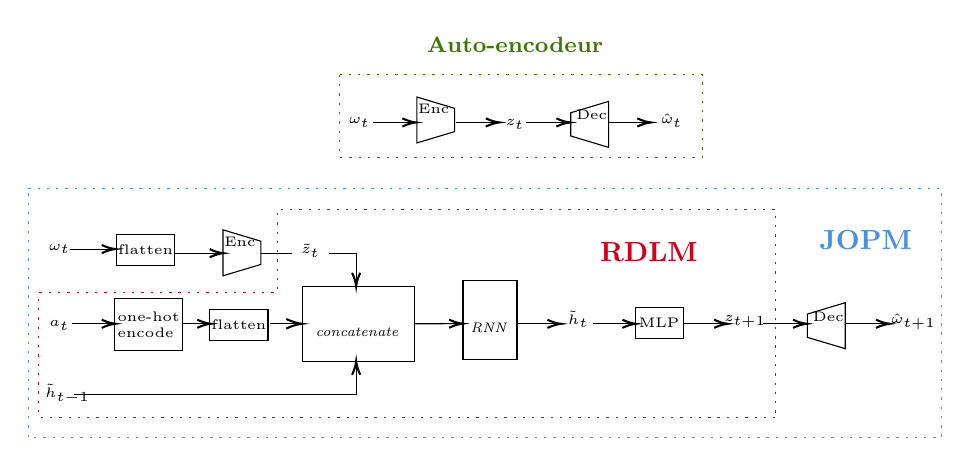
\begin{tikzpicture}[x=0.75pt,y=0.75pt,yscale=-1,xscale=1]
    %uncomment if require: \path (0,2102); %set diagram left start at 0, and has height of 2102

    %Straight Lines [id:da7905055997256106] 
    \draw    (53.06,1235.47) -- (73.06,1235.47) ;
    \draw [shift={(75.06,1235.47)}, rotate = 180] [color={rgb, 255:red, 0; green, 0; blue, 0 }  ][line width=0.75]    (6.56,-1.97) .. controls (4.17,-0.84) and (1.99,-0.18) .. (0,0) .. controls (1.99,0.18) and (4.17,0.84) .. (6.56,1.97)   ;
    %Straight Lines [id:da5451220917566785] 
    \draw    (54.23,1271.47) -- (73.06,1271.47) ;
    \draw [shift={(75.06,1271.47)}, rotate = 180] [color={rgb, 255:red, 0; green, 0; blue, 0 }  ][line width=0.75]    (6.56,-1.97) .. controls (4.17,-0.84) and (1.99,-0.18) .. (0,0) .. controls (1.99,0.18) and (4.17,0.84) .. (6.56,1.97)   ;
    %Straight Lines [id:da4433866589105997] 
    \draw    (55.06,1305.47) -- (191.06,1305.47) -- (191.06,1291.47) ;
    \draw [shift={(191.06,1289.47)}, rotate = 90] [color={rgb, 255:red, 0; green, 0; blue, 0 }  ][line width=0.75]    (6.56,-1.97) .. controls (4.17,-0.84) and (1.99,-0.18) .. (0,0) .. controls (1.99,0.18) and (4.17,0.84) .. (6.56,1.97)   ;
    %Straight Lines [id:da9772153219599438] 
    \draw    (107.06,1271.47) -- (119.06,1271.47) ;
    \draw [shift={(121.06,1271.47)}, rotate = 180] [color={rgb, 255:red, 0; green, 0; blue, 0 }  ][line width=0.75]    (6.56,-1.97) .. controls (4.17,-0.84) and (1.99,-0.18) .. (0,0) .. controls (1.99,0.18) and (4.17,0.84) .. (6.56,1.97)   ;
    %Straight Lines [id:da08798558878605356] 
    \draw    (149.44,1271.47) -- (163.06,1271.47) ;
    \draw [shift={(165.06,1271.47)}, rotate = 180] [color={rgb, 255:red, 0; green, 0; blue, 0 }  ][line width=0.75]    (7.65,-2.3) .. controls (4.86,-0.97) and (2.31,-0.21) .. (0,0) .. controls (2.31,0.21) and (4.86,0.98) .. (7.65,2.3)   ;
    %Straight Lines [id:da5508296944602415] 
    \draw    (103.06,1237.47) -- (125.06,1237.47) ;
    \draw [shift={(127.06,1237.47)}, rotate = 180] [color={rgb, 255:red, 0; green, 0; blue, 0 }  ][line width=0.75]    (6.56,-1.97) .. controls (4.17,-0.84) and (1.99,-0.18) .. (0,0) .. controls (1.99,0.18) and (4.17,0.84) .. (6.56,1.97)   ;
    %Shape: Trapezoid [id:dp14410290094148615] 
    \draw   (126.9,1226.21) -- (145.13,1231.68) -- (145.13,1242.88) -- (126.9,1248.35) -- cycle ;
    %Straight Lines [id:da384443735490001] 
    \draw    (145.06,1237.47) -- (191.06,1237.47) -- (191.06,1251.47) ;
    \draw [shift={(191.06,1253.47)}, rotate = 270] [color={rgb, 255:red, 0; green, 0; blue, 0 }  ][line width=0.75]    (6.56,-1.97) .. controls (4.17,-0.84) and (1.99,-0.18) .. (0,0) .. controls (1.99,0.18) and (4.17,0.84) .. (6.56,1.97)   ;
    %Straight Lines [id:da5196284966358902] 
    \draw    (219.06,1271.47) -- (240.39,1271.41) ;
    \draw [shift={(242.39,1271.41)}, rotate = 179.85] [color={rgb, 255:red, 0; green, 0; blue, 0 }  ][line width=0.75]    (6.56,-1.97) .. controls (4.17,-0.84) and (1.99,-0.18) .. (0,0) .. controls (1.99,0.18) and (4.17,0.84) .. (6.56,1.97)   ;
    %Straight Lines [id:da2885650017773205] 
    \draw    (268.95,1271.5) -- (287.78,1271.5) ;
    \draw [shift={(289.78,1271.5)}, rotate = 180] [color={rgb, 255:red, 0; green, 0; blue, 0 }  ][line width=0.75]    (6.56,-1.97) .. controls (4.17,-0.84) and (1.99,-0.18) .. (0,0) .. controls (1.99,0.18) and (4.17,0.84) .. (6.56,1.97)   ;
    %Straight Lines [id:da1683388835537969] 
    \draw    (305.06,1271.47) -- (323.89,1271.47) ;
    \draw [shift={(325.89,1271.47)}, rotate = 180] [color={rgb, 255:red, 0; green, 0; blue, 0 }  ][line width=0.75]    (6.56,-1.97) .. controls (4.17,-0.84) and (1.99,-0.18) .. (0,0) .. controls (1.99,0.18) and (4.17,0.84) .. (6.56,1.97)   ;
    %Straight Lines [id:da18138221495614015] 
    \draw    (349.06,1271.47) -- (356.46,1271.47) -- (368.1,1271.47) ;
    \draw [shift={(370.1,1271.47)}, rotate = 180] [color={rgb, 255:red, 0; green, 0; blue, 0 }  ][line width=0.75]    (6.56,-1.97) .. controls (4.17,-0.84) and (1.99,-0.18) .. (0,0) .. controls (1.99,0.18) and (4.17,0.84) .. (6.56,1.97)   ;
    %Shape: Trapezoid [id:dp15428640042958097] 
    \draw   (426.67,1283.47) -- (408.44,1278) -- (408.44,1266.79) -- (426.67,1261.32) -- cycle ;
    %Straight Lines [id:da8308982689158874] 
    \draw    (387.06,1271.47) -- (406.1,1271.47) ;
    \draw [shift={(408.1,1271.47)}, rotate = 180] [color={rgb, 255:red, 0; green, 0; blue, 0 }  ][line width=0.75]    (6.56,-1.97) .. controls (4.17,-0.84) and (1.99,-0.18) .. (0,0) .. controls (1.99,0.18) and (4.17,0.84) .. (6.56,1.97)   ;
    %Straight Lines [id:da854779381814783] 
    \draw    (427.06,1271.47) -- (446.1,1271.47) ;
    \draw [shift={(448.1,1271.47)}, rotate = 180] [color={rgb, 255:red, 0; green, 0; blue, 0 }  ][line width=0.75]    (6.56,-1.97) .. controls (4.17,-0.84) and (1.99,-0.18) .. (0,0) .. controls (1.99,0.18) and (4.17,0.84) .. (6.56,1.97)   ;
    %Shape: Trapezoid [id:dp12236333694521873] 
    \draw   (220.29,1162.21) -- (238.52,1167.68) -- (238.52,1178.88) -- (220.29,1184.35) -- cycle ;
    %Shape: Trapezoid [id:dp4232724503855386] 
    \draw   (312.67,1186.47) -- (294.44,1181) -- (294.44,1169.79) -- (312.67,1164.32) -- cycle ;
    %Straight Lines [id:da0811328179216142] 
    \draw    (313.06,1174.47) -- (331.06,1174.47) ;
    \draw [shift={(333.06,1174.47)}, rotate = 180] [color={rgb, 255:red, 0; green, 0; blue, 0 }  ][line width=0.75]    (6.56,-1.97) .. controls (4.17,-0.84) and (1.99,-0.18) .. (0,0) .. controls (1.99,0.18) and (4.17,0.84) .. (6.56,1.97)   ;
    %Straight Lines [id:da33212985731507805] 
    \draw    (199.06,1174.47) -- (217.89,1174.47) ;
    \draw [shift={(219.89,1174.47)}, rotate = 180] [color={rgb, 255:red, 0; green, 0; blue, 0 }  ][line width=0.75]    (6.56,-1.97) .. controls (4.17,-0.84) and (1.99,-0.18) .. (0,0) .. controls (1.99,0.18) and (4.17,0.84) .. (6.56,1.97)   ;
    %Straight Lines [id:da7950301814204398] 
    \draw    (239.06,1174.47) -- (258.1,1174.47) ;
    \draw [shift={(260.1,1174.47)}, rotate = 180] [color={rgb, 255:red, 0; green, 0; blue, 0 }  ][line width=0.75]    (6.56,-1.97) .. controls (4.17,-0.84) and (1.99,-0.18) .. (0,0) .. controls (1.99,0.18) and (4.17,0.84) .. (6.56,1.97)   ;
    %Straight Lines [id:da8317125190119203] 
    \draw    (273.06,1174.47) -- (292.1,1174.47) ;
    \draw [shift={(294.1,1174.47)}, rotate = 180] [color={rgb, 255:red, 0; green, 0; blue, 0 }  ][line width=0.75]    (6.56,-1.97) .. controls (4.17,-0.84) and (1.99,-0.18) .. (0,0) .. controls (1.99,0.18) and (4.17,0.84) .. (6.56,1.97)   ;
    %Shape: Polygon [id:ds33250073085001886] 
    \draw  [color={rgb, 255:red, 208; green, 2; blue, 27 }  ,draw opacity=1 ][dash pattern={on 0.84pt off 2.51pt}] (393.06,1316.47) -- (38.06,1316.47) -- (38.06,1256.47) -- (153.06,1256.47) -- (153.06,1216.47) -- (393.06,1216.47) -- cycle ;
    %Shape: Rectangle [id:dp3415456817493894] 
    \draw  [color={rgb, 255:red, 74; green, 144; blue, 226 }  ,draw opacity=1 ][dash pattern={on 0.84pt off 2.51pt}] (33.06,1206.47) -- (473.06,1206.47) -- (473.06,1326.47) -- (33.06,1326.47) -- cycle ;
    %Shape: Rectangle [id:dp9296059531842202] 
    \draw  [color={rgb, 255:red, 65; green, 117; blue, 5 }  ,draw opacity=1 ][dash pattern={on 0.84pt off 2.51pt}] (183.06,1151.47) -- (358.06,1151.47) -- (358.06,1191.47) -- (183.06,1191.47) -- cycle ;


    % Text Node
    \draw (332.06,1236.97) node  [color={rgb, 255:red, 208; green, 2; blue, 27 }  ,opacity=1 ] [align=left] {\textbf{RDLM}};
    % Text Node
    \draw (436.56,1230.97) node  [color={rgb, 255:red, 74; green, 144; blue, 226 }  ,opacity=1 ] [align=left] {\textbf{JOPM}};
    % Text Node
    \draw (267.56,1136.97) node  [color={rgb, 255:red, 65; green, 117; blue, 5 }  ,opacity=1 ] [align=left] {{\footnotesize \textbf{Auto-encodeur}}};
    % Text Node
    \draw (192.56,1174.47) node  [font=\tiny] [align=left] {$\displaystyle \omega _{t}$};
    % Text Node
    \draw (343.06,1173.47) node  [font=\tiny] [align=left] {$\displaystyle \hat{\omega }_{t}$};
    % Text Node
    \draw (304.56,1170.97) node   [align=left] {{\tiny Dec}};
    % Text Node
    \draw (228.44,1167.97) node   [align=left] {{\tiny Enc}};
    % Text Node
    \draw (267.56,1175.47) node  [font=\tiny] [align=left] {$\displaystyle z_{t}$};
    % Text Node
    \draw (459.6,1270.47) node  [font=\tiny] [align=left] {$\displaystyle \hat{\omega }_{t+1}$};
    % Text Node
    \draw (418.56,1267.97) node   [align=left] {{\tiny Dec}};
    % Text Node
    \draw (378.56,1270.47) node  [font=\tiny] [align=left] {$\displaystyle z_{t+1}$};
    % Text Node
    \draw (135.06,1231.97) node   [align=left] {{\tiny Enc}};
    % Text Node
    \draw (298.06,1269.47) node  [font=\tiny] [align=left] {$\displaystyle \tilde{h}_{t}$};
    % Text Node
    \draw    (242.54,1250.47) -- (268.54,1250.47) -- (268.54,1288.47) -- (242.54,1288.47) -- cycle  ;
    \draw (255.54,1269.47) node  [font=\tiny] [align=left] {\begin{minipage}[lt]{14.99pt}\setlength\topsep{0pt}
            \begin{center}
                \phantom{X}\\\textit{RNN}
            \end{center}

        \end{minipage}};
    % Text Node
    \draw  [color={rgb, 255:red, 255; green, 255; blue, 255 }  ,draw opacity=1 ][fill={rgb, 255:red, 255; green, 255; blue, 255 }  ,fill opacity=1 ]  (160.56,1227.47) -- (177.56,1227.47) -- (177.56,1245.47) -- (160.56,1245.47) -- cycle  ;
    \draw (169.06,1236.47) node  [font=\tiny] [align=left] {$\displaystyle \tilde{z}_{t}$};
    % Text Node
    \draw    (165.06,1253.47) -- (219.06,1253.47) -- (219.06,1289.47) -- (165.06,1289.47) -- cycle  ;
    \draw (192.06,1271.47) node  [font=\tiny] [align=left] {\begin{minipage}[lt]{34pt}\setlength\topsep{0pt}
            \begin{center}
                \phantom{X}\\\textit{concatenate}
            \end{center}

        \end{minipage}};
    % Text Node
    \draw    (120.56,1264.47) -- (148.56,1264.47) -- (148.56,1279.47) -- (120.56,1279.47) -- cycle  ;
    \draw (134.56,1271.97) node  [font=\tiny] [align=left] {flatten};
    % Text Node
    \draw (52.06,1305.47) node  [font=\tiny] [align=left] {$\displaystyle \tilde{h}_{t-1}$};
    % Text Node
    \draw (48.06,1272.47) node  [font=\tiny] [align=left] {$\displaystyle a_{t}$};
    % Text Node
    \draw (48.06,1235.47) node  [font=\tiny] [align=left] {$\displaystyle \omega _{t}$};
    % Text Node
    \draw    (325.56,1263.47) -- (348.56,1263.47) -- (348.56,1278.47) -- (325.56,1278.47) -- cycle  ;
    \draw (337.06,1270.97) node  [font=\tiny] [align=left] {MLP};
    % Text Node
    \draw    (74.56,1259.47) -- (107.56,1259.47) -- (107.56,1284.47) -- (74.56,1284.47) -- cycle  ;
    \draw (91.06,1271.97) node  [font=\tiny] [align=left] {one-hot\\encode};
    % Text Node
    \draw    (75.56,1228.47) -- (103.56,1228.47) -- (103.56,1243.47) -- (75.56,1243.47) -- cycle  ;
    \draw (89.56,1235.97) node  [font=\tiny] [align=left] {flatten};


\end{tikzpicture}
  }
  \caption{Schematic of the architecture of a JOPM including the RLDM and the Auto-encoder.}
  \label{fig:jopm_architecture}
\end{figure}

% \widetilde{\hat{\omega }}_{t}

More precisely, each joint observation $\omega_t^{j} = (\omega_t^1, \dots, \omega_t^{|\mathcal{A}|}) \in \Omega^{j}$ is flattened into a single vector $\tilde{\omega}_t = vec (\omega_t^1, \dots, \omega_t^{|\mathcal{A}|})$, then passed through an encoder $Enc~: \tilde{\Omega}\rightarrow Z$ to produce a latent representation $z_t = Enc(\tilde{\omega}_t)$. A decoder $Dec~: Z \rightarrow \widetilde{\hat{\Omega}}$ allows the flattened joint observation $\widetilde{\hat{\omega}}_t = Dec(z_t)$ to be reconstructed before being recomposed into an approximate joint observation $\hat{\omega}_t^{j} = unvec(\widetilde{\hat{\omega}}_t) = (\hat{\omega}_t^1, \dots, \hat{\omega}_t^{|\mathcal{A}|}) \in \Omega^ {j}$.

MLPs or attention-based architectures are generally used for the autoencoder (encoder-decoder set) in order to aggregate multi-agent information into fixed-size feature vectors while capturing critical dependencies between agents.

Once encoding has been performed on the set of joint observations $\omega^j \in \Omega^{j}$ to obtain the latent representations $z_t \in Z_t$, the multi-agent World Model operates as in a single-agent context, using the encoded observations $z_t$ in the histories transmitted to the \textbf{RLDM} $\mathcal{T}^{z}$; an \textbf{RLDM} can also be used. For each of the collected episodes $h^j \in \mathcal{D}_{H^j} $, for each step $t \in \llbracket 0, n_{step} \rrbracket$, the latent representation of the joint observation $z_t$ is concatenated with the recurrent hidden state vector $\tilde{h}_{t-1}$ and the flattened joint action vector $\tilde{a}_t$. The vector resulting from this concatenation is passed through the \textbf{RNN} (\textbf{LSTM}) to update the recurrent hidden state vector $\tilde{h}_{t}$ and then passed through an \textbf{MLP} to determine the latent representation of the approximate joint observation at the next time step $z_{t+1} $. Next, the decoder $Dec$ is used to reconstruct the flattened approximate joint observation $\tilde{\hat{\omega}}_{t+1}^{j}$. Finally, this flattened approximate joint observation is recomposed into a predicted joint observation for the next state $\hat{\omega}_{t+1}^{j}$.


\section{Neuro-Symbolic Multi-Agent WMs}
\label{sec:method}

We propose \emph{Neuro-Symbolic Multi-Agent WMs (NS-MAWM)}, a framework... TODO... A schematic overview of NS-MAWM is provided in \autoref{fig:ns-mawm_overview}.

% \begin{figure}[t]
%   \centering
%   % In the preamble (if not already present):
% \usepackage{tikz}
% \usetikzlibrary{arrows.meta,positioning,fit,calc}

\begin{figure}[t]
    \centering

    \resizebox{\textwidth}{!}{%

        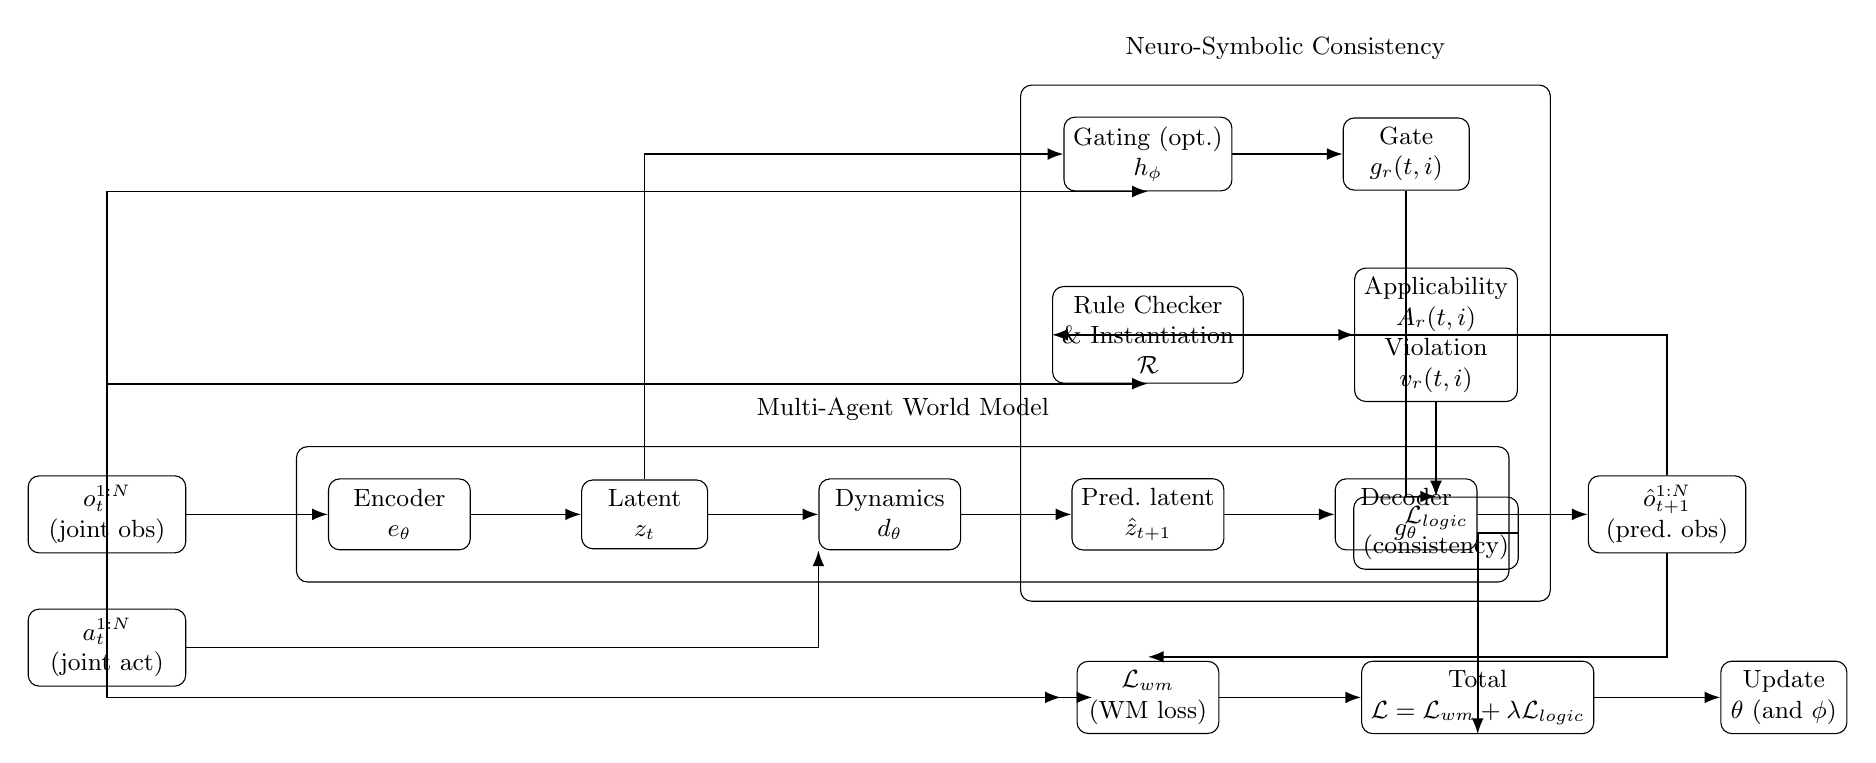
\begin{tikzpicture}[
                font=\small,
                node distance=10mm and 14mm,
                box/.style={draw, rounded corners, align=center, minimum height=9mm, minimum width=18mm},
                smallbox/.style={draw, rounded corners, align=center, minimum height=8mm, minimum width=16mm},
                io/.style={draw, rounded corners, align=center, fill=white, minimum height=8mm, minimum width=20mm},
                loss/.style={draw, rounded corners, align=center, minimum height=9mm, minimum width=18mm},
                group/.style={draw, rounded corners, inner sep=4mm},
                arr/.style={-Latex, line width=0.6pt}
            ]

            % ====== Main WM pipeline ======
            \node[io] (obs) {$o_t^{1:N}$\\(joint obs)};
            \node[io, below=7mm of obs] (act) {$a_t^{1:N}$\\(joint act)};

            \node[box, right=18mm of obs] (enc) {Encoder\\$e_\theta$};
            \node[smallbox, right=14mm of enc] (zt) {Latent\\$z_t$};

            \node[box, right=14mm of zt] (dyn) {Dynamics\\$d_\theta$};
            \node[smallbox, right=14mm of dyn] (znext) {Pred.\ latent\\$\hat z_{t+1}$};

            \node[box, right=14mm of znext] (dec) {Decoder\\$g_\theta$};
            \node[io, right=14mm of dec] (opred) {$\hat o_{t+1}^{1:N}$\\(pred.\ obs)};

            % arrows main
            \draw[arr] (obs) -- (enc);
            \draw[arr] (enc) -- (zt);
            \draw[arr] (zt) -- (dyn);
            \draw[arr] (dyn) -- (znext);
            \draw[arr] (znext) -- (dec);
            \draw[arr] (dec) -- (opred);

            % action into dynamics
            \draw[arr] (act) -| (dyn.south west);

            % ====== Losses ======
            \node[loss, below=14mm of znext] (lwm) {$\mathcal{L}_{wm}$\\(WM loss)};
            \draw[arr] (opred.south) |- ($(lwm.north)+(0,0.5mm)$);
            \draw[arr] (obs.south)  |- ($(lwm.west)+(-2mm,0)$); % indicates supervision / target
            \draw[arr] (act.south)  |- ($(lwm.west)+(2mm,0)$);

            % ====== Neuro-symbolic constraint path ======
            \node[box, above=12mm of znext] (rules) {Rule Checker\\\& Instantiation\\$\mathcal{R}$};
            \node[smallbox, right=14mm of rules] (viol) {Applicability\\$A_r(t,i)$\\Violation\\$v_r(t,i)$};

            \draw[arr] (opred.north) |- (rules.west);
            \draw[arr] (act.north)  |- (rules.south);
            \draw[arr] (rules) -- (viol);

            % gating (optional)
            \node[box, above=12mm of rules] (gate) {Gating (opt.)\\$h_\phi$};
            \node[smallbox, right=14mm of gate] (gcoef) {Gate\\$g_r(t,i)$};

            \draw[arr] (zt.north) |- (gate.west);
            \draw[arr] (act.north) |- (gate.south);
            \draw[arr] (gate) -- (gcoef);

            % logic loss
            \node[loss, below=12mm of viol] (llogic) {$\mathcal{L}_{logic}$\\(consistency)};
            \draw[arr] (viol) -- (llogic);
            \draw[arr] (gcoef) |- (llogic.north);

            % total objective
            \node[loss, right=18mm of lwm] (ltot) {Total\\$\mathcal{L}=\mathcal{L}_{wm}+\lambda\mathcal{L}_{logic}$};
            \draw[arr] (lwm) -- (ltot);
            \draw[arr] (llogic) -| (ltot.south);

            % parameter update annotation
            \node[smallbox, right=16mm of ltot] (upd) {Update\\$\theta$ (and $\phi$)};
            \draw[arr] (ltot) -- (upd);

            % ====== Group boxes (optional, for readability) ======
            \node[group, fit=(enc)(zt)(dyn)(znext)(dec), label={[yshift=2mm]above:Multi-Agent World Model}] (wmgroup) {};
            \node[group, fit=(rules)(viol)(gate)(gcoef)(llogic), label={[yshift=2mm]above:Neuro-Symbolic Consistency}] (nsgroup) {};

        \end{tikzpicture}}

    \caption{Overview of NS-MAWM. A multi-agent world model encodes joint observations, predicts latent dynamics conditioned on joint actions, and decodes predicted observations. Neuro-symbolic rules are instantiated on predictions to compute applicability and violation scores; an optional gating network modulates rule enforcement. Training minimizes $\mathcal{L}_{wm} + \lambda \mathcal{L}_{logic}$.}
    \label{fig:overview}
\end{figure}

%   \caption{Overview of the NS-MAWM framework: ...TODO}
%   \label{fig:ns-mawm_overview}
% \end{figure}

\subsection{Structured observation latent space and unified neuro-symbolic formalism}
\label{sec:ns}

TODO

\subsection{The three neuro-symbolic integration strategies}
\label{sec:integration_strategies}

\subsubsection{The symbolic loss regularization strategy}
\label{sec:symbolic_loss_regularization}

TODO

\subsubsection{The symbolic projection strategy}
\label{sec:symbolic_projection}

TODO

\subsubsection{The residual symbolic dynamics strategy}
\label{sec:residual_symbolic_dynamics}

TODO

\subsection{Rule Violation Rate (RVR)}
\label{sec:rvr}

TODO

\subsection{NS-MAWM global algorithm}
\label{sec:algo}

TODO

% ============================
\section{Evaluation}
\label{sec:eval}

This section evaluates... TODO

\subsection{Implementation}
\label{sec:impl_overview}

TODO...

\subsection{Environments and rule sets}
\label{sec:envs}

We consider two classes of environments: ... TODO

\subsection{Computing resources and hyperparameters}
\label{sec:resources}

TODO

\subsection{Evaluation metrics, baselines and protocol}
\label{sec:metrics_baselines_protocol}
% Comment on fait pour évaluer que NS-MAWM est mieux que les autres et permet d'atteindre les objectifs fixés dans l'intro :
%  - est-ce qu'on prend mieux en compte l'aspect multi-agent ?
%  - est-ce qu'on réduit le drift sémantique sur le long terme grâce à l'intégration symbolique ? Si oui, comment ?
%  - est-ce que ça améliore la performance en planification / RL downstream ?
%  - est-ce que ça améliore la généralisation à de nouvelles configurations d'agents/objets ?
%  - est-ce que ça améliore l'efficacité des données (moins de données nécessaires pour atteindre une certaine performance) ?
%  - est-ce qu'on peut faire une ablation pour montrer l'importance de chaque composant (invariants vs equivariances, stratégies d'intégration, etc.) ?
%  - est-ce qu'on peut tester la robustesse aux règles incomplètes ou incorrectes ?
%  - est-ce qu'on peut tester la scalabilité avec le nombre d'agents/règles ?
%  - est-ce qu'on peut évaluer correctement les performances avec des métriques symboliques (RVR) en plus des métriques classiques (log-likelihood, erreur de reconstruction, récompense downstream) ?

% 1) donner les métriques utilisées
% 2) présenter les baselines comparées pour permettre d'évaluer l'apport de NS-MAWM
% 3) expliquer le protocole expérimental (nombre de seeds, durée d'entraînement, etc.) afin de fournir un moyen scientifique de voir si on couvre bien les gaps identifiés dans l'intro en faisant le lien avec les métriques et baselines via le protocole expérimental

TODO

\subsection{Results}
\label{sec:results}

TODO

% ============================
% 7. Conclusion
% ============================
\section{Conclusion and future work}
\label{sec:conclusion}

TODO

\section*{Impact Statement}

This paper presents work whose goal is to advance the field of Machine Learning by improving the reliability of model-based multi-agent reinforcement learning.
By reducing semantic inconsistencies in learned WMs, this work may contribute to safer and more interpretable decision-making in multi-agent systems.
We do not identify ethical concerns specific to this work beyond those commonly associated with reinforcement learning research.


% ============================
% Acknowledgements (remove for submission if needed)
% ============================
% \section*{Acknowledgements}

% ============================
% References
% ============================
\bibliography{references}
\bibliographystyle{icml2026}

%%%%%%%%%%%%%%%%%%%%%%%%%%%%%%%%%%%%%%%%%%%%%%%%%%%%%%%%%%%%%%%%%%%%%%%%%%%%%%%
%%%%%%%%%%%%%%%%%%%%%%%%%%%%%%%%%%%%%%%%%%%%%%%%%%%%%%%%%%%%%%%%%%%%%%%%%%%%%%%
% APPENDIX
%%%%%%%%%%%%%%%%%%%%%%%%%%%%%%%%%%%%%%%%%%%%%%%%%%%%%%%%%%%%%%%%%%%%%%%%%%%%%%%
%%%%%%%%%%%%%%%%%%%%%%%%%%%%%%%%%%%%%%%%%%%%%%%%%%%%%%%%%%%%%%%%%%%%%%%%%%%%%%%

\newpage

\appendix

\section{Rule Set Details}
\label{app:rules}
% TODO:
% - list rules formally
% - applicability masks
% - examples

\section{Additional Experimental Results}
\label{app:more}
% TODO:
% - ablations, extra environments, hyperparams

\section{Architectures and Hyperparameters}
\label{app:hparams}
% TODO:
% - full hyperparam tables

%%%%%%%%%%%%%%%%%%%%%%%%%%%%%%%%%%%%%%%%%%%%%%%%%%%%%%%%%%%%%%%%%%%%%%%%%%%%%%%
%%%%%%%%%%%%%%%%%%%%%%%%%%%%%%%%%%%%%%%%%%%%%%%%%%%%%%%%%%%%%%%%%%%%%%%%%%%%%%%

\end{document}

% This document was modified from the file originally made available by
% Pat Langley and Andrea Danyluk for ICML-2K. This version was created
% by Iain Murray in 2018, and modified by Alexandre Bouchard in
% 2019 and 2021 and by Csaba Szepesvari, Gang Niu and Sivan Sabato in 2022.
% Modified again in 2023 and 2024 by Sivan Sabato and Jonathan Scarlett.
% Previous contributors include Dan Roy, Lise Getoor and Tobias
% Scheffer, which was slightly modified from the 2010 version by
% Thorsten Joachims & Johannes Fuernkranz, slightly modified from the
% 2009 version by Kiri Wagstaff and Sam Roweis's 2008 version, which is
% slightly modified from Prasad Tadepalli's 2007 version which is a
% lightly changed version of the previous year's version by Andrew
% Moore, which was in turn edited from those of Kristian Kersting and
% Codrina Lauth. Alex Smola contributed to the algorithmic style files.
